\documentclass{standalone}
\usepackage{tikz}
\usetikzlibrary{automata, positioning}


\newcommand{\nodeStyle}[0]{
  % Setup the style for the states
  \tikzset{
    node style/.style={
    state, 
    minimum width=2cm,
    line width=1mm,
    fill={rgb:red,1;green,0;blue,0}}
  }
}

\newcommand{\createNode}[4]{
  \node[node style] at (#3,#4)(#1){#2};
}


\begin{document}
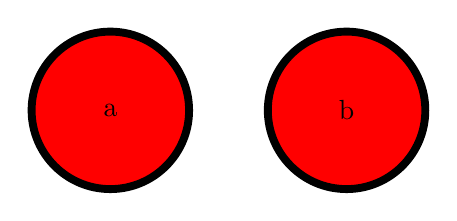
\begin{tikzpicture}

  \nodeStyle
  \createNode{a}{a}{0}{0}
  \createNode{b}{b}{3}{0}


\end{tikzpicture}
\end{document}

